\section{Design}

\subsection{System-level design}
The complete system will consist of energy harvesting source, energy storage for times when harvested energy is not available, AC/DC and DC/DC converters for maintaining required voltage levels in different blocks of system, accelerometer for measuring the accleration in tyre and bluetooth/microcontroller module for transmitting data from acceleromoter. Figure \ref{system_blog_diagram} shows the power and data flow between subsections of system. 


\begin{figure}[htb]
\begin{center}
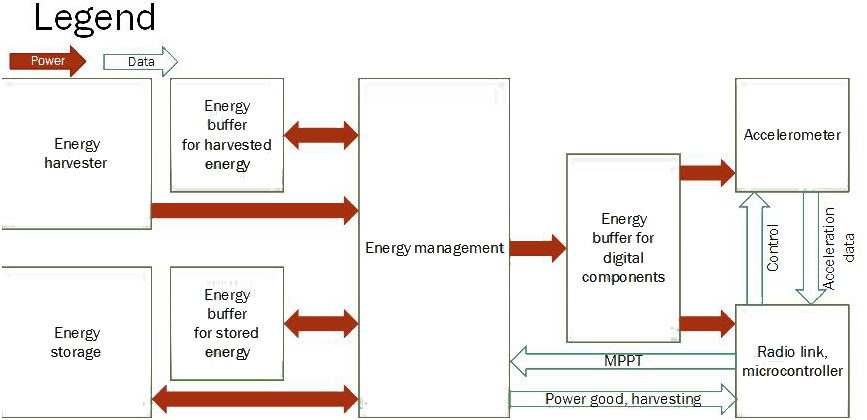
\includegraphics[height=6cm]{images/system_block_diagram.jpg}
\end{center}
\caption{\label{system_blog_diagram} Block diagram of complete system.}
\label{liitekuva}
\end{figure}


\subsection{Electrical design}
The analog sections of circuit were simulated using LTSpice IV {\color{red} reference}. Accelerometer and bluetooth module were modelled as parallel current sinks which took energy from the circuit in pulses. Energy harvesting was simulated as a high.impedance AC voltage source. 
Battery was modelled as a voltage source with high-value capacitor and low-value resistor in series.

\subsection{Overview of usable energy harvesting methods}
Several different methods for harvesting were experimented with to find optimal solution for the application. After background study on chapter {\color{red} refer to background} of energy harvesting methods, it was obvious that methods which use mechanical energy as their power source are best suited to application. Different approaches are piezoelectronic, electrostatic, electromagnetic and microelectromechanical systems (MEMS). 

Piezoelectronic systems use {\color{red} review of physical basis of piezos}.  The elements are stackable, so power output can be scaled as needed if higher cost of system is allowable. Their power output is rather limited, and it is uncertain if usable output of a few milliwatts could be reached with element stack of reasonable size and cost.

Electrostatic devices charge plates of capacitor and use mechanical vibration to vary the structure of a capacitor. As the capacitance value changes with the structure, energy can be harvested from increased potential energy in capacitor. Drawback of this method is the required control electronics and high polarization voltages needed for maximal efficiency {\color{red} cite Electrostatic conversion for Vibration Energy harvesting}. There are also electrostatic methods which use *electrets*, Electronic Magnets {\color{red} cite}. These electrects hold constant charge and polarization for years and they can be used in electrostatic harvesters which do not require an external exitation source. While electrostatic harvesters have reached the required power levels, they are not readily available at the moment. Vibration characteristics of tyre pose additional challenges to electrostatic harvesters, as the plates must be protected against contact to one another during shocks. {\color{red} cite}

Electromagnetic harvesters utilise vibration to move a magnet inside a coil. The movement of a magnet causes a changing magnetic field, which gets coupled to coil. Coil opposes the change in magnetic field by inducing electrical current in device. {\color{red} cite} A device could be built with a spring-loaded magnet to balance out the static acceleration of a tyre. An added bonus to spring loaded mechanism would be the utilisation of resonant frequency of the spring-mass system: as the system gets a shock, some of the energy would be in correct frequency range to make the magnet oscillate inside coil allowing generation of energy until next shock. The coil will also function  as a dampener to system, so no extra dampening is required. Primary concern is the survivability of a magnet in an environment with heavy shocks and vibration. 

An in-depth overview is done to piezoelectric and electromagnetic methods, as they are best fits to environment and previous work has proved it's possible to generate required amounts of power with both methods.{\color{red} cite}

\subsubsection{Resonant piezoelectric harvesting}
A common approach to piezoelectric harvesting is to configure the element as a cantilever and tune the resonant frequency of the system to dominant frequency of the surrounding environment. This tuning is done by attaching a mass to the end of cantilever. This sort of tuned approach is not feasible in the environment of the tire, as the piezoelectric harvester has to be compliant enough to vibrate in low accelerations of few g's and stiff enough to withstand centripetal shocks of several hundred g's. {\color{red} Cite}. 

\subsubsection{Impact based piezoelectric harvesting}
As the resonant harvesting is not feasible in the environment inside tire, another method would be to use an impactor to hit a piezoelectric plate on every cycle of a tire. These impacts would provide energy once per rotation of a tire. This method has been tried before by {\color{red} Cite} and it was found to provide up to 4 mW of power in average. 

\subsubsection{Electromagnetical harvesting}
As the electromagnetical harvester does not bend in any direction, it's better suited to be built straight up along Z-axis. The structure can be made strong enough to survive the shocks present without compromising on the harvester operation. A magnet can be suspended with a spring inside a coil. When there is vibration in addition to relatively constant centripetal force, the magnet will move along the shaft of the coil and generate electricity.

A non-linear spring can be utilised to keep the magnet as well centered as possible over a wide range of tyre speeds. Theoretically this non-linearity could also be used to shift the resonant frequency of generator to track the frequency of vibration inside the tyre. In practise the movement of magnet would drive the spring outside of the resonant area. 

\subsection{Electromagnetical harvester design}
A theoretical design of linear generator was made. Most common generator designs use a rotating magnet inside coils to generate alternating current. As the mechanical apparatus for converting the linear accelerations inside tire to rotational movement would add to complexity and cost of the tire, generator is design to use the linear motion as the power source.

Basic principle of operation is similar to traditional rotational generator. A moving magnet creates alternating magnetic field which is coupled to coiled conductors. The conductors oppose this change of magnetic field by inducing an electrical current across their ends. The design can have multiple phases and poles. Multiple phase designs can be made smaller and lighter at the expense of more complex control circuitry. {\color{red} cite}. 

Adding poles to design increases the output voltage {\color{red} cite a study of multi-pole} and frequency, but having a small airgap between the coils and magnets becomes critical to maintain efficiency of the generator. 

A simulink model was built to verify feasibility of the linear generator. The model included real acceleration data from previous studies made by {\color{red} cite} and a model of generator as well as a simplified capacitive-resistive load. There is an abundance of previous work done on simulating linear generators  {\color{red} cite}, however a simplified model was used at this stage to get a proof-of-concept level generator. Further work remains in optimizing the design in terms of size, mass, power output, usable speed range, cost and long-term reliability.

First design decision was whether to use a moving magnet or moving coil type of a design. Moving coil designs tend to have lighter moving parts which is a very important feature in high-power designs where mass of the generator is large. On the other hand, moving coil require flying leads  {\color{red} cite development of a moving magnet linear}.  which is a long-term reliability concern  {\color{red} cite linear electric actuators and generators}.  {\color{red} cite book Boldea, Nasar Linear electric actuators and generators p 203}. conclude that moving coil designs aren't practically interesting, so the design is focused on moving magnet generator. 

A rough model for designing initial prototypes was done previously by  {\color{red} cite backpack harvester}. As the work verified the model experimentally and found the model to be reasonably accurate, it was adapted to form basis of linear generator model. The model can account for most of the key design parameters. 

\begin{table}[htb]
%% Taulukon teksti
\caption{\label{parameters_of_lg} Effect of parameters of generator}
\begin{center}
\fbox{
\begin{tabular}{l l l}
\textbf{Parameter}		& \textbf{Increasing} 		& \textbf{Decreasing}	\\ \hline
Number of turns in generator	& Higher voltage		& Smaller size, less wiring resistance 		\\ \hline
Number of poles			& Increased frequency		& Decreased frequency	\\ \hline
Distance between poles  	& More space for wiring 	& Higher voltage, smaller size	\\ \hline
Wiring radius		  	& More power			& Smaller length of wiring 	\\ \hline
Magnetic field strength  	& Increased power 		& Smaller magnets 		\\ \hline
Wire diameter		  	& Decreased wiring resistance 	& More turns in same space 	\\ \hline
Gap to wiring			& Stronger side walls		& Incresed efficiency 
\end{tabular}
}
\end{center}
\end{table}

Energy harvester designs often use several poles to increase the frequency of the power output {\color{red}cite}. This increased frequency allows to use smaller energy storage components such as capacitors to keep the device powered until next cycle. The characteristics of the tyre make this point a moot, as energy is available once per revolution of the tire when generator contacts the ground and when the contact ends. Any energy storage device has to maintain power until the next cycle, and no increase of the frequency while generator is in contact can alleviate that. Therefore number of poles is minimized to reduce complexity. Pole number is selected as two, so there is one negative and one positive pole. 

There are two different approaches to generator structure. One is magnets inside, and coils on the outer rim of the generator. Other is to use ring magnets on the outer rim and have the coils on the inside. Both methods have their advantages: Having magnets on the outside allows larger and therefore stronger magnets and creates horizontal support for the magnets as they slide along the shaft. Having coils on the outside increases wiring radius which results in greater power if other parameters are held equal. In-depth study of both concepts is done to select optimal structure for generator. 

The height of the generator is constrained at  {\color{yellow} confirm} 45 mm. Initially the height of {\color{gray} the} generator was selected to be 35-40 mm to leave some margin while still being as tall as possible. Lower weight is desirable to avoid unbalancing the tyre, but there is no specific absolute maximum mass for the device. 

A method to counter the centripetal acceleration is needed to avoid jamming the magnet on the bottom of the generator. Ideally, such method would always balance the magnet in the middle of generator against any external constant force, but active control is not achievable without adding to complexity and power consumption of the generator itself. Passive negative feedback method has to be used instead. 

Springs are often chosen {\color{red} cite few sources} to balance the magnets, but as the centripetal acceleration grows exponentially with the speed of the car, any linear spring would be usable only for very limited range of speeds. Non-linear conical springs which have the added benefit of compressing into very small height are available.

Another approach would be to use two additional magnets fixed to top and bottom of the generator in repulsive configuration. Force between magnets is inversely propotional to fourth power of the distance {\color{red} cite}, which leads to a strong negative feedback on the position of the magnet. 

Magnetic floating is very attaractive solution, as magnets can be very thin and they do not wear out with aging. On the other hand, any imbalance in the magnets result in torgue which causes increased friction. {\color{yellow} picture?} This issue is further aggravated in designs where shape of the generator shaft is not a smooth cylinder. Therefore the design should have any grooves filled with suitable epoxy and the shaft should be sanded or turned to final diameter to ensure smooth sliding across the length of shaft.

\subsection{Materials for the harvester}
Material for the shaft has a few requirements. It has to have at least as good temperature characteristics as the magnet being used and it must be hard enough to not deform under impacts. Low friction coefficient is desirable as this leads to smaller losses, and long time durability under wear is of course desired. Being lightweight and easily machinable are also desired characteristics. As the generator is small, volumetric cost of the material is of little concern. For the electro-magnetic generator design material also has to be non-ferromagnetic {\color{red} verify?}. Table {\color{yellow} refer?} has comparison of different materials considered for the application.

\begin{table}[htb]
%% Taulukon teksti
\caption{\label{parameters_of_materials} Materials for the shaft of generator}
\begin{center}
\fbox{
\begin{tabular}{l l l l l l}
\textbf{Material}& 
\textbf{Hardness \cite{PlasticsInternational2015}}& 
\textbf{Friction \cite{Etra}} & 
\textbf{Durability \cite{Etra}} & 
\textbf{Temperature \cite{Etra}}\\ \hline
PTFE(Teflon)      & Very low   & Lowest                      & Lowest    & -190... + 250 \degree C \\ \hline
Polycarbonate     & Very high  & High  \cite{Goodfellow}     & -         & -60... + 125 \degree C \\ \hline
PA 6 (Nylon)      & Low        & Medium                      & High      & -40... + 80 \degree C  \\ \hline
Oil-infused Nylon & Low        & Very low                    & Very high & -20... + 105 \degree C \\ \hline
Acryllic          & High       & -                           & -         & -40... + 70 \degree C \\ \hline
Polyacetal (POM C)& Medium     & Low                         & Low       & -50... + 105 \degree C \\ \hline
\end{tabular}
}
\end{center}
\end{table}
